\chapter{Reglas de fabricación y de diseño}\label{cap:jlc}
% nombre de regla que se puede partir en los guiones bajos (solo en este capítulo)
\providecommand{\regla}[1]{\texttt{#1}}

Antes de dibujar una sola pista hay que saber \emph{qué puede fabricar} la fábrica y \emph{qué reglas se
quieren cumplir} en el diseño. Este capítulo explica las dos cosas y cómo se cargaron en KiCad para que el
programa avise solo cuando algo no se cumple.

En este capítulo vas a ver:
\begin{itemize}
  \item cómo se fabrica una placa de circuito impreso, lo justo para entender de dónde salen las reglas;
  \item las capacidades de JLCPCB que usamos y cuánto margen dejamos sobre cada mínimo;
  \item qué es una vía taponada y por qué obligó a mover 43 vías;
  \item qué pide el ensamblaje \emph{Economic} de JLC (rieles, fiduciales, distancia al borde);
  \item el acabado HASL sin plomo y lo que cuesta;
  \item cómo se tradujo todo a KiCad: restricciones de placa, clases de red y las reglas propias del archivo
        \archivo{pcb.kicad_dru};
  \item qué son los \emph{teardrops} y por qué se pusieron.
\end{itemize}

Las fuentes de todo el capítulo están en \archivo{hardware/pcb/REGLAS.md} (secciones 1, 2, 8 y 9), en
\archivo{pcb.kicad_pro}, en \archivo{pcb.kicad_dru} y en \archivo{tools/config_reglas.py}, que es el script que
escribe la configuración.

% =====================================================================================================
\section{Cómo se fabrica una PCB (lo justo para entender las reglas)}\label{sec:c06-fabricacion}

Una PCB es un ``sándwich'' de capas de cobre separadas por material aislante (FR-4, fibra de vidrio con resina
epóxica). Nuestra placa tiene \textbf{4 capas de cobre}: dos por fuera (\capa{F.Cu} arriba y \capa{B.Cu} abajo) y
dos por dentro (\capa{In1.Cu} e \capa{In2.Cu}). En el capítulo~\ref{cap:capas} se explica por qué terminó en 4
capas; aquí solo importa cómo se fabrica.

Los pasos, simplificados, son estos:
\begin{enumerate}
  \item \textbf{Grabado del cobre.} Se parte de láminas de FR-4 cubiertas de cobre. Se protege con una película
        fotosensible lo que debe quedar (pistas, pads, planos) y el resto se disuelve con químicos. El grabado no
        es perfecto: el ácido también ``muerde'' un poco por los lados. Por eso existe un \textbf{ancho mínimo de
        pista} y una \textbf{separación mínima} entre cobres.
  \item \textbf{Laminado.} En una placa de 4 capas, primero se graban las capas internas sobre un núcleo
        (\emph{core}). Luego se apilan con hojas de pre-impregnado (\emph{prepreg}) y las láminas de cobre
        externas, y se prensan en caliente.
  \item \textbf{Taladrado.} Una broca hace los agujeros de las vías y de los pines de los componentes con agujero
        pasante (THT). La broca tiene un diámetro mínimo y su posición tiene una tolerancia: el agujero nunca cae
        exactamente en el centro del pad. De ahí salen el \textbf{anillo anular mínimo} (cuánto cobre debe quedar
        alrededor del agujero) y la \textbf{distancia mínima de un agujero a otro cobre}.
  \item \textbf{Metalizado.} Las paredes de los agujeros se recubren de cobre. Así un agujero une eléctricamente
        las capas que atraviesa: eso es una \emph{vía} (si solo sirve para cambiar de capa) o un pad PTH (si además
        lleva un pin).
  \item \textbf{Máscara de soldadura.} Es la resina verde. Cubre todo el cobre menos los lugares donde se va a
        soldar (aperturas). Entre dos aperturas vecinas queda una tira delgada de máscara, el \textbf{puente de
        máscara}, que evita que la soldadura corra de un pad al otro. Esa tira tiene un ancho mínimo.
  \item \textbf{Acabado superficial.} El cobre que queda expuesto se protege para que no se oxide y se pueda
        soldar. Nosotros elegimos \textbf{HASL sin plomo}: la placa se sumerge en estaño fundido y un chorro de
        aire caliente nivela la superficie.
  \item \textbf{Serigrafía.} Tinta blanca con los nombres de las piezas (designadores), marcas de pin 1 y de
        polaridad. La impresión tiene una resolución limitada: \textbf{alto y grosor mínimos de texto}.
  \item \textbf{Fresado del contorno.} Una fresa corta la placa con su forma final. La fresa no puede pasar
        pegada al cobre sin dañarlo: hay una \textbf{distancia mínima de cobre a borde}.
\end{enumerate}

La figura~\ref{fig:c06-corte} muestra un corte de la placa con esas partes. Los espesores están exagerados para
que se vean; los reales son los del apilado JLC04161H-7628 \doc{JLC, página de impedancia}: cobre externo
\SI{0.035}{\milli\meter}, prepreg 7628 de \SI{0.2104}{\milli\meter}, cobre interno \SI{0.0152}{\milli\meter} y núcleo
de \SI{1.065}{\milli\meter}, para un total de \SI{1.6}{\milli\meter}.

\begin{figure}[htbp]
\centering
\begin{tikzpicture}[x=1cm,y=1cm,font=\small]
  % espesores exagerados; y = 0 abajo
  \fill[green!45!black!70] (0,0) rectangle (9,0.2);                % máscara inferior
  \fill[orange!70!brown] (0,0.2) rectangle (3.95,0.45);            % B.Cu (GND) con holgura alrededor de la vía
  \fill[orange!70!brown] (4.95,0.2) rectangle (9,0.45);
  \fill[orange!70!brown] (4.15,0.2) rectangle (4.75,0.45);         % anillo de la vía abajo
  \fill[yellow!25] (0,0.45) rectangle (9,1.25);                    % prepreg
  \fill[orange!70!brown] (0,1.25) rectangle (4.75,1.5);            % In2: pista de la misma red que la vía
  \fill[orange!70!brown] (5.35,1.25) rectangle (9,1.5);            % In2: otra red, con holgura
  \fill[yellow!45] (0,1.5) rectangle (9,3.3);                      % núcleo
  \fill[orange!70!brown] (0,3.3) rectangle (3.95,3.55);            % In1 GND con holgura alrededor de la vía
  \fill[orange!70!brown] (4.95,3.3) rectangle (9,3.55);
  \fill[yellow!25] (0,3.55) rectangle (9,4.35);                    % prepreg
  \fill[orange!70!brown] (0.6,4.35) rectangle (2.2,4.6);           % pista F.Cu
  \fill[orange!70!brown] (4.15,4.35) rectangle (4.75,4.6);         % anillo de la vía arriba
  \fill[orange!70!brown] (6.6,4.35) rectangle (8.0,4.6);           % pad SMD
  \fill[gray!45] (6.7,4.6) rectangle (7.9,4.78);                   % estaño HASL
  \fill[green!45!black!70] (0,4.6) rectangle (6.35,4.85);          % máscara superior (cubre la vía)
  \fill[green!45!black!70] (8.25,4.6) rectangle (9,4.85);
  \fill[white,draw=black,line width=0.3pt] (2.6,4.85) rectangle (3.5,5.02); % serigrafía
  % vía: paredes metalizadas y tapón
  \fill[orange!70!brown] (4.15,0.2) rectangle (4.25,4.6);
  \fill[orange!70!brown] (4.65,0.2) rectangle (4.75,4.6);
  \fill[gray!25] (4.25,0.3) rectangle (4.65,4.5);
  % rótulos de arriba (dos filas)
  \begin{scope}[font=\footnotesize]
    \draw[-{Latex[length=1.6mm]}] (1.4,5.65) node[above]{pista} -- (1.4,4.65);
    \draw[-{Latex[length=1.6mm]}] (4.45,5.65) node[above]{vía taponada} -- (4.45,4.9);
    \draw[-{Latex[length=1.6mm]}] (7.3,5.65) node[above]{pad con HASL} -- (7.3,4.82);
    \draw[-{Latex[length=1.6mm]}] (3.05,6.35) node[above]{serigrafía} -- (3.05,5.06);
    \draw[-{Latex[length=1.6mm]}] (5.85,6.35) node[above]{máscara de soldadura} -- (5.85,4.88);
  \end{scope}
  % rótulos de la derecha
  \draw[-{Latex[length=1.6mm]}] (10,4.47) node[right]{\capa{F.Cu} (\SI{35}{\micro\meter})} -- (8.9,4.47);
  \draw[-{Latex[length=1.6mm]}] (10,3.95) node[right]{prepreg 7628} -- (8.9,3.95);
  \draw[-{Latex[length=1.6mm]}] (10,3.42) node[right]{\capa{In1.Cu}: plano GND} -- (8.9,3.42);
  \draw[-{Latex[length=1.6mm]}] (10,2.4) node[right]{núcleo FR-4} -- (8.9,2.4);
  \draw[-{Latex[length=1.6mm]}] (10,1.37) node[right]{\capa{In2.Cu}} -- (8.9,1.37);
  \draw[-{Latex[length=1.6mm]}] (10,0.85) node[right]{prepreg 7628} -- (8.9,0.85);
  \draw[-{Latex[length=1.6mm]}] (10,0.32) node[right]{\capa{B.Cu}} -- (8.9,0.32);
  \draw[-{Latex[length=1.6mm]}] (10,-0.35) node[right]{máscara inferior} -- (8.9,0.1);
  % holgura del plano
  \draw[-{Latex[length=1.6mm]}] (2.2,2.75) node[below,font=\footnotesize,align=center]{el plano GND se aparta\\de la vía (holgura)} -- (4.0,3.38);
\end{tikzpicture}
\caption{Corte esquemático de la placa de 4 capas (espesores no a escala). La vía atraviesa las cuatro capas; en
\capa{In1.Cu} y en \capa{B.Cu} el cobre de GND le deja una holgura porque la vía es de otra red, y en \capa{In2.Cu} se une a una pista
de su misma red. El agujero de la vía queda relleno de tinta (taponado) y cubierto de máscara.}
\label{fig:c06-corte}
\end{figure}

\begin{idea}[por qué hay mínimos]
Cada paso tiene una tolerancia: el ácido se come un poco de más, la broca cae un poco corrida, la máscara se
imprime un poco desplazada. Los ``mínimos'' de la fábrica son los valores con los que todavía garantizan que, con
esas tolerancias, la placa sale bien. Si diseñas \emph{justo} en el mínimo, cualquier desviación te deja al borde
del error. Por eso en este diseño casi todo se hizo con \textbf{valores de diseño mayores que el mínimo}: los
mínimos quedaron solo como piso de seguridad en KiCad.
\end{idea}

% =====================================================================================================
\section{Las capacidades de JLCPCB que usamos}\label{sec:c06-capacidades}

La fábrica es JLCPCB (China), porque además fabrica y \emph{ensambla} la placa con piezas de su propio catálogo
(LCSC). Sus capacidades se leyeron en sus páginas el 15 y el 16 de noviembre de 2026
\doc{jlcpcb.com/capabilities/pcb-capabilities}. La tabla~\ref{tab:c06-capacidades} resume cada mínimo, lo que se
puso en KiCad como piso y lo que se usó de verdad en el diseño.

Una aclaración importante: la configuración se escribió primero para \textbf{2 capas}, porque la placa empezó así.
Cuando se pasó a 4 capas, los mínimos de JLC para placas multicapa resultaron iguales o \emph{menores} que los de
2 capas (por ejemplo, pista y separación de \SI{0.09}{\milli\meter} en vez de \SI{0.10}{\milli\meter}). Por eso los
pisos de 2 capas se dejaron: siguen siendo válidos y son un poco más conservadores. Lo que sí hubo que agregar
fueron las reglas propias de las capas internas (sección~\ref{sec:c06-dru}).

{\small
\begin{longtable}{@{}L{0.25\linewidth}L{0.22\linewidth}L{0.13\linewidth}L{0.33\linewidth}@{}}
\caption{Capacidades de JLCPCB, piso en KiCad y valor de diseño. Fuentes: REGLAS.md §1 y §9
\doc{páginas de capacidades de JLC}.}\label{tab:c06-capacidades}\\
\toprule
\textbf{Concepto} & \textbf{Mínimo de JLC} & \textbf{Piso en KiCad} & \textbf{Valor de diseño y margen}\\
\midrule\endfirsthead
\toprule
\textbf{Concepto} & \textbf{Mínimo de JLC} & \textbf{Piso en KiCad} & \textbf{Valor de diseño y margen}\\
\midrule\endhead
Ancho de pista & \SI{0.10}{\milli\meter} (2 capas); \SI{0.09}{\milli\meter} (multicapa, \SI{1}{\oz}) & \SI{0.10}{\milli\meter}
  & \SI{0.2}{\milli\meter} en señales; \SI{0.25}{\milli\meter} o más en potencia. El doble del mínimo.\\
Separación pista–pista & \SI{0.10}{\milli\meter} / \SI{0.09}{\milli\meter} & \SI{0.10}{\milli\meter}
  & \SI{0.2}{\milli\meter}; \SI{0.3}{\milli\meter} en analógicas y relojes.\\
Pad–pad SMD (redes distintas) & \SI{0.15}{\milli\meter} & — & \SI{0.2}{\milli\meter} (regla \net{pad_a_pad}).\\
Vía (taladro / diámetro) & \SI{0.15}{\milli\meter} / \SI{0.25}{\milli\meter} & igual
  & \SI{0.3}{\milli\meter} / \SI{0.6}{\milli\meter}. JLC no cobra recargo con taladro $\geq$ \SI{0.3}{\milli\meter}
  \doc{cotizador JLC}.\\
Anillo de vía & \SI{0.05}{\milli\meter} (\SI{0.075}{\milli\meter} preferido) & \SI{0.10}{\milli\meter}
  & \SI{0.15}{\milli\meter} (ver el cálculo de abajo). Tres veces el mínimo.\\
Anillo de pad PTH & \SI{0.18}{\milli\meter} absoluto, \SI{0.25}{\milli\meter} recomendado (2 capas);
  \SI{0.15}{\milli\meter} mínimo, \SI{0.20}{\milli\meter} recomendado (4 capas) & regla \net{anillo_pth}: \SI{0.20}{\milli\meter}
  & lo fija cada footprint; en los Gerber el anillo mínimo medido es \SI{0.150}{\milli\meter}, que es el de las
  vías (sección~\ref{sec:c06-dru}).\\
Agujero de vía a pista & \SI{0.20}{\milli\meter} & \SI{0.20}{\milli\meter} & $\geq$ \SI{0.35}{\milli\meter} (anillo más separación).\\
Agujero PTH a pista & \SI{0.28}{\milli\meter} (\SI{0.35}{\milli\meter} recomendado) & \SI{0.28}{\milli\meter} (regla propia)
  & $\geq$ \SI{0.55}{\milli\meter}.\\
Taladro de vía a cobre interno & \SI{0.2}{\milli\meter} & regla propia & igual al mínimo, verificado por el DRC.\\
Taladro de PTH a cobre interno & \SI{0.3}{\milli\meter} & regla propia & igual al mínimo, verificado por el DRC.\\
Agujero a agujero & \SI{0.2}{\milli\meter} (vías) / \SI{0.45}{\milli\meter} (pads) & \SI{0.25}{\milli\meter} & —\\
Cobre a borde & $\geq$ \SI{0.2}{\milli\meter} & \SI{0.20}{\milli\meter} & \SI{0.5}{\milli\meter} (regla \net{borde}).\\
Puente de máscara (verde) & \SI{0.10}{\milli\meter} & — & $\geq$ \SI{0.25}{\milli\meter} en todos los footprints.\\
Apertura de máscara & 1:1 con el pad; $\geq$ \SI{0.09}{\milli\meter} a pistas vecinas & máscara–cobre \SI{0.09}{\milli\meter}
  & expansión 0 (apertura del tamaño del pad).\\
Serigrafía & línea $\geq$ \SI{0.15}{\milli\meter}; texto $\geq$ \SI{1.0}{\milli\meter}; $\geq$ \SI{0.15}{\milli\meter} a pads
  & texto \SI{1.0}{\milli\meter} / \SI{0.15}{\milli\meter} & \SI{1.0}{\milli\meter} de alto, \SI{0.15}{\milli\meter} de trazo, solo
  \ang{0} y \ang{90}.\\
Cobre interno & \SI{0.5}{\oz} por defecto & — & \SI{0.5}{\oz} (\SI{15.2}{\micro\meter}).\\
\bottomrule
\end{longtable}
}

\begin{calculo}[anillo anular de nuestra vía]
La vía de diseño tiene un pad de \SI{0.6}{\milli\meter} de diámetro y un taladro de \SI{0.3}{\milli\meter}. El anillo
es el cobre que queda alrededor del agujero, de un solo lado:
\[
  \text{anillo} = \frac{D_\text{pad} - D_\text{taladro}}{2} = \frac{\num{0.6} - \num{0.3}}{2} = \SI{0.15}{\milli\meter}.
\]
JLC pide \SI{0.05}{\milli\meter} (\SI{0.075}{\milli\meter} preferido). Aunque la broca caiga corrida
\SI{0.1}{\milli\meter}, todavía queda cobre alrededor. La revisión de los Gerber con gerbonara midió exactamente ese
\SI{0.150}{\milli\meter} como anillo mínimo de la placa \medido.
\end{calculo}

\begin{ojo}[mínimo no es objetivo]
En KiCad hay dos lugares donde se pone un ancho: el mínimo de la placa y el valor de la clase de red. Si pones el
valor de JLC en la clase, el programa te deja dibujar todo al límite. En este diseño los valores de JLC van
\emph{solo} en el mínimo (para que el DRC proteja) y los de diseño en las clases. Así lo dice la nota de
REGLAS.md §1: ``los valores de la última columna van en las clases de red y en \archivo{pcb.kicad_dru}, nunca en el
mínimo''.
\end{ojo}

% =====================================================================================================
\section{Vías tapadas y vías taponadas}\label{sec:c06-vias}

Una vía es un agujero metalizado. Si queda abierto, al soldar el estaño se puede ir por el agujero y robarle
soldadura a un pad vecino, o puede quedar químico atrapado. Hay varias formas de cubrirlo:
\begin{itemize}
  \item \textbf{Tented} (tapada): la máscara pasa por encima del agujero como una tela. Es lo normal en 2 capas.
  \item \textbf{Plugged} (taponada): el agujero se rellena con tinta y luego se cubre con máscara. Es más
        robusto.
\end{itemize}

En el cotizador de JLC, para \textbf{4 capas} la opción por defecto es \emph{Plugged}: si pides \emph{Tented},
ellos la pasan a \emph{Plugged} sin costo \doc{cotizador JLC}. Eso trae una condición que no existía en 2 capas.
JLC escribe: ``vias with a distance less than 0.35mm from the pad cannot be plugged with ink''
\doc{jlcpcb.com/help/article/pcb-via-covering}. Es decir, una vía a menos de \SI{0.35}{\milli\meter} de un pad no se
puede taponar.

\begin{decision}[vías a \SI{0.35}{\milli\meter} o más de los pads]
\textbf{Qué se decidió:} toda vía queda a \SI{0.35}{\milli\meter} o más de cualquier pad, incluso de un pad de su
misma red. Se creó la regla \net{via_tapada_lejos_de_pad} en \archivo{pcb.kicad_dru}.

\textbf{Alternativas:} pedir vías abiertas o pagar un relleno epóxico (otra opción del cotizador), o dejar las vías
pegadas al pad y aceptar que JLC no las tapone.

\textbf{Por qué:} el desacoplo ideal pone la vía de GND ``pegada'' al pad del condensador, y muchas vías estaban
así. Pero una vía mal taponada junto a un pad es justo el caso que se quiere evitar al soldar. Cuando se midió con
una regla de prueba, 43 de las 59 vías que había en ese momento estaban a menos de \SI{0.35}{\milli\meter} de algún
pad. El dueño decidió correrlas, y se movieron 43 vías de los bloques 1, 3 y 4 (\archivo{PLAN_RUTEO.md} §11.1). En
algunos casos la vía pasó debajo del cuerpo del condensador; en otro (C19) no había ningún lugar legal y ese
condensador se une a tierra por el relleno de GND de \capa{F.Cu} (es una de las excepciones del
capítulo~\ref{cap:banco}).

\textbf{Fuente:} JLC, artículo de recubrimiento de vías y página de capacidades (``should have $\geq$ 0.35 mm
clearance from other soldermask openings'').
\end{decision}

Además, en la configuración de la placa todas las vías van cubiertas de máscara en las dos caras y ninguna lo anula.
Esto se comprobó en los archivos de fabricación: la revisión de los Gerber cuenta \textbf{329 vías} de
\SI{0.3}{\milli\meter} y \textbf{0 aperturas de máscara} sobre ellas, arriba y abajo \medido{}
(\archivo{fabricacion/revision_gerber.md}).

\begin{idea}[por qué \emph{physical\_clearance} y no \emph{clearance}]
La regla normal de separación (\emph{clearance}) de KiCad solo mira cobres de \emph{redes distintas}: entre una vía
de GND y un pad de GND no hay nada que separar. Pero el problema del taponado es físico, no eléctrico: no importa la
red, importa la distancia. Por eso la regla usa \emph{physical\_clearance}, que KiCad aplica también entre objetos de
la misma red.
\end{idea}

% =====================================================================================================
\section{Ensamblaje: PCBA \emph{Economic}}\label{sec:c06-pcba}

JLC ofrece dos servicios de ensamblaje (PCBA) \doc{cotizador y página de capacidades de PCBA}:
\begin{itemize}
  \item \textbf{Economic}: monta piezas en \emph{una sola cara}. Junta pedidos de varios clientes y los produce
        juntos, por eso es barato (la página habla de un costo de preparación de \$8). Placa mínima de
        \num{10} $\times$ \SI{10}{\milli\meter}.
  \item \textbf{Standard}: una o dos caras, sin límite de cantidad, pero la placa debe medir al menos
        \num{70} $\times$ \SI{70}{\milli\meter} y los rieles son obligatorios.
\end{itemize}

Nuestra placa mide \num{90} $\times$ \SI{64}{\milli\meter}: con \SI{64}{\milli\meter} de alto no entra en
\emph{Standard} sin panelizar, pero sí en \emph{Economic}. Todas las piezas SMD van en la cara de arriba
(\capa{F.Cu}), así que \emph{Economic} sirve.

\subsection{Distancia del cuerpo de las piezas al borde, rieles y fiduciales}

La máquina de montaje sujeta la placa por los bordes. Por eso JLC pide que el \textbf{cuerpo} de las piezas quede a
\SI{2.5}{\milli\meter} o más del borde si la placa no tiene rieles \doc{JLC, PCBA}. En nuestra placa no se cumple en
el borde superior, donde están los bucks:

\begin{center}
\begin{tabular}{@{}lc@{}}
\toprule
\textbf{Piezas} & \textbf{Cuerpo a borde}\\
\midrule
\net{L1}, \net{L2} (bobinas) & \SI{1.30}{\milli\meter}\\
\net{C31}--\net{C34}, \net{C41}--\net{C44} (condensadores de salida) & \SI{1.35}{\milli\meter}\\
\net{R33}, \net{C47} (filtro de 5V\_A) & \SI{1.85}{\milli\meter}\\
\bottomrule
\end{tabular}
\end{center}

\begin{decision}[rieles agregados por JLC]
\textbf{Qué se decidió:} no tocar el contorno ni el placement; pedir que JLC agregue los rieles.

\textbf{Alternativas:} correr el bloque de bucks hacia abajo (rompía el placement de todo el bloque de potencia, que
ya estaba revisado), o dibujar rieles propios en \capa{Edge.Cuts}.

\textbf{Por qué:} los términos de JLC dicen que, si la placa no trae rieles ni fiduciales, ellos los agregan por
defecto. En el cotizador aparece igual: ``If there are no edge rails or fiducials in your design, JLC will help to
add them by default''. Con los rieles, el borde ``real'' de la máquina queda lejos de las piezas.

\textbf{Fuente:} términos del servicio de ensamblaje de JLC y texto del cotizador (REGLAS.md §2).
\end{decision}

Los \textbf{fiduciales} son círculos de cobre desnudo que la cámara de la máquina usa para saber dónde está la placa
con precisión. JLC pide cobre de \SI{1}{\milli\meter} con \SI{2}{\milli\meter} de apertura de máscara, 3 o 4 cerca de
los bordes, a \SI{3.35}{\milli\meter} o más del borde \doc{JLC, PCBA}. Se pusieron tres, \net{FID1} a \net{FID3}, con
el footprint \net{Fiducial_1mm_Mask2mm}, en $(\num{4.5}, \num{5})$, $(\num{82}, \num{6})$ y
$(\num{16}, \num{44})$~\si{\milli\meter} desde la esquina inferior izquierda. Tienen el atributo \emph{board only}:
existen en la placa pero no en el esquemático, ni en el BOM ni en el archivo de posiciones (CPL). Tres puntos que no
están en línea bastan para corregir posición, giro y escala.

\subsection{La combinación que vamos a pedir sí cabe en \emph{Economic}}

No todas las combinaciones de placa se pueden pedir con \emph{Economic}. El 16 de noviembre se leyó la tabla de la
página de capacidades de PCBA con el navegador, incluida la columna de capas
\doc{jlcpcb.com/capabilities/pcb-assembly-capabilities}:

\begin{center}
\begin{tabular}{@{}ccccc@{}}
\toprule
\textbf{Capas} & \textbf{Espesor} & \textbf{Máscara} & \textbf{Acabado} & \textbf{Cantidad de placas}\\
\midrule
4L & \SI{1.6}{\milli\meter} & Green & Lead-Free: HASL / ENIG & 2--50\\
\bottomrule
\end{tabular}
\end{center}

Es exactamente lo que se va a pedir: 4 capas, \SI{1.6}{\milli\meter}, verde, HASL sin plomo, 5 placas. La misma
página dice ``Standard stack-up only'', y el apilado JLC04161H-7628 es el estándar de 4 capas.

\begin{ojo}[cantidad a ensamblar, sin confirmar]
Lo que falta confirmar es \emph{cuántas} de las 5 placas deja ensamblar \emph{Economic}. El cotizador no muestra
esa opción hasta subir los Gerber, y en su demo \emph{Economic} aparece deshabilitado; con \emph{Standard}, la demo
permite ``Qty from 2 to 5''. Esto importa porque la bobina \net{L2} tenía solo 4 unidades en stock el 16/11: la
decisión fue ensamblar como máximo 4 placas. Si \emph{Economic} solo ofrece 2 o 5, se ensamblan 2. Se confirma al
armar el pedido.
\end{ojo}

\subsection{Los archivos que pide JLC}
JLC tiene una guía de exportación para KiCad. En resumen (REGLAS.md §2):
\begin{itemize}
  \item \textbf{Gerber}: formato Protel, X2, coordenadas 4.6 en milímetros; capas de cobre, máscara, serigrafía,
        pasta y \capa{Edge.Cuts}. Antes de exportar se rellenan las zonas.
  \item \textbf{Taladros}: Excellon, milímetros, origen absoluto, archivos PTH y NPTH separados.
  \item \textbf{BOM}: columnas \emph{Comment, Designator, Footprint, LCSC Part Number}.
  \item \textbf{CPL} (posiciones): \emph{Designator, Mid X, Mid Y, Layer, Rotation}, con la rotación positiva en
        sentido antihorario. JLC no publica una tabla de correcciones de giro, así que la rotación se corrigió pieza
        por pieza; eso se explica en el capítulo~\ref{cap:verif}.
\end{itemize}

% =====================================================================================================
\section{Acabado HASL sin plomo y precio}\label{sec:c06-acabado}

Las opciones de acabado que se compararon, con su precio para 5 placas de \num{90} $\times$
\SI{64}{\milli\meter}, 4 capas, \SI{1.6}{\milli\meter} y máscara verde (cotizador de JLC sin sesión, sin envío ni
ensamblaje, 16/11/2026) \doc{cotizador JLC}:

\begin{center}
\begin{tabular}{@{}lrL{0.52\linewidth}@{}}
\toprule
\textbf{Acabado} & \textbf{Precio} & \textbf{Qué es}\\
\midrule
HASL con plomo & USD 8.00 (oferta) & estaño-plomo; el más barato\\
\textbf{HASL sin plomo} & \textbf{USD 13.20} & aleación sin plomo (cumple RoHS)\\
ENIG & USD 25.30 & níquel y una capa fina de oro: superficie muy plana\\
\bottomrule
\end{tabular}
\end{center}

\begin{decision}[HASL sin plomo]
\textbf{Qué se decidió:} HASL sin plomo (decisión del dueño, 16/11/2026, registrada en
\archivo{fabricacion/LEEME.md}).

\textbf{Alternativas:} HASL con plomo (USD 5.20 más barato con la oferta) o ENIG (casi el doble).

\textbf{Argumentos:} el HASL sin plomo cumple RoHS y evita manipular plomo al retocar o al soldar a mano las piezas
THT (borneras, BNC, zócalo de la NUCLEO). ENIG da una superficie más plana; el propio cotizador dice que el HASL es un
poco irregular y conviene menos con piezas de paso muy fino. Aquí el paso más fino es el de los bucks
(\SI{0.5}{\milli\meter}), no hay BGA, y la tabla de \emph{Economic} admite HASL para esta placa. La diferencia de unos
USD 12 frente a ENIG no se consideró justificada.

\textbf{Fuente:} cotizador de JLC (REGLAS.md §9) y descripción de acabados del propio cotizador.
\end{decision}

% =====================================================================================================
\section{Cómo se cargó todo esto en KiCad}\label{sec:c06-kicad}

KiCad tiene tres lugares donde se ponen las reglas. Conviene entender la diferencia:

\begin{enumerate}
  \item \textbf{Restricciones de la placa} (\emph{Board Setup → Constraints}): son el \emph{piso absoluto}. Nada en
        la placa puede estar por debajo, sea de la red que sea.
  \item \textbf{Clases de red} (\emph{Net Classes}): agrupan redes parecidas y les dan su ancho de pista, su
        separación y su vía \emph{de diseño}. Cuando trazas una pista de esa red, KiCad usa esos valores.
  \item \textbf{Reglas propias} (archivo \archivo{pcb.kicad_dru}): reglas escritas a mano con condiciones, para lo
        que no cabe en las dos anteriores (por ejemplo, ``las redes de reloj a \SI{0.5}{\milli\meter} de las
        analógicas'').
\end{enumerate}

Las tres las escribe el script \archivo{tools/config_reglas.py}, que modifica \archivo{pcb.kicad_pro} y genera
\archivo{pcb.kicad_dru}. Tenerlo en un script tiene una ventaja: si algo se daña, se vuelve a generar igual, y el
script documenta de dónde sale cada número.

\subsection{Restricciones de la placa}
Valores leídos en \archivo{pcb.kicad_pro} \medido:

\begin{center}
\begin{tabular}{@{}L{0.34\linewidth}L{0.26\linewidth}L{0.32\linewidth}@{}}
\toprule
\textbf{Restricción} & \textbf{Valor} & \textbf{Comentario}\\
\midrule
Separación mínima & \SI{0.10}{\milli\meter} & JLC 2 capas\\
Ancho mínimo de pista & \SI{0.10}{\milli\meter} & JLC 2 capas\\
Vía mínima (diámetro / taladro) & \SI{0.25}{\milli\meter} / \SI{0.15}{\milli\meter} & JLC\\
Anillo mínimo de vía & \SI{0.10}{\milli\meter} & decisión: JLC permite \SI{0.05}{\milli\meter}\\
Agujero a cobre & \SI{0.20}{\milli\meter} & JLC, vía a pista\\
Agujero a agujero & \SI{0.25}{\milli\meter} & JLC \SI{0.2}{\milli\meter} entre vías\\
Cobre a borde & \SI{0.20}{\milli\meter} & JLC; el diseño usa \SI{0.5}{\milli\meter} por regla\\
Serigrafía a serigrafía & \SI{0.05}{\milli\meter} & solo detecta solapes (ver regla \net{serigrafia_a_pad})\\
Alto / grosor de texto & \SI{1.0}{\milli\meter} / \SI{0.15}{\milli\meter} & JLC\\
Máscara a cobre & \SI{0.09}{\milli\meter} & JLC\\
\bottomrule
\end{tabular}
\end{center}

\subsection{Clases de red}
Una \emph{red} es un conjunto de pines unidos eléctricamente (por ejemplo, \net{IEPE_SV}). Las clases agrupan las
redes que se tratan igual. Los valores de diseño son los de la tabla~\ref{tab:c06-clases}.

\begin{table}[htbp]
\centering\small
\caption{Clases de red del proyecto (\archivo{pcb.kicad_pro} y \archivo{tools/config_reglas.py}).}
\label{tab:c06-clases}
\begin{tabularx}{\linewidth}{@{}lcccY@{}}
\toprule
\textbf{Clase} & \textbf{Ancho} & \textbf{Separación} & \textbf{Vía} & \textbf{Redes}\\
\midrule
Default & \SI{0.2}{\milli\meter} & \SI{0.2}{\milli\meter} & 0.6/0.3 & I2C, straps del PCM1808 (MD/FMT), BOOT, FB y VCC de los bucks\\
Potencia & \SI{0.25}{\milli\meter} & \SI{0.2}{\milli\meter} & 0.6/0.3 & \net{24V_IN}, \net{24V_PROT}, \net{3V3}, \net{5V},
  \net{5V_A}, \net{GND}, \net{IEPE_SUP*}, \net{3V3_DAC*}\\
Conmutado & \SI{0.25}{\milli\meter} & \SI{0.2}{\milli\meter} & 0.6/0.3 & \net{SW_3}, \net{SW_5} (nodos de conmutación de los bucks)\\
Analogica & \SI{0.2}{\milli\meter} & \SI{0.3}{\milli\meter} & 0.6/0.3 & \net{IEPE*}, \net{REST*}, \net{DC_MON*}, \net{SUM},
  divisores, \net{DAC_F}, \net{VSHIFT}, entradas del ADC, \net{VREF}, SET/OUT de los LT3092\\
Reloj & \SI{0.2}{\milli\meter} & \SI{0.3}{\milli\meter} & 0.6/0.3 & \net{SAI_*}, BCK/LRCK/DOUT/SCKI del PCM1808, salida de \net{Y1}\\
\bottomrule
\end{tabularx}
\end{table}

Algunas cosas que conviene notar:
\begin{itemize}
  \item \textbf{Analógica y Reloj tienen más separación} (\SI{0.3}{\milli\meter}): son las redes sensibles al ruido y
        las que más ruido generan. Más separación entre pistas vecinas significa menos acople capacitivo.
  \item \textbf{Potencia empezó en \SI{0.5}{\milli\meter}} con vía de 0.8/0.4. Después del bloque 1 el dueño pidió
        que la clase tuviera los valores \emph{reales} del ruteo: \SI{0.25}{\milli\meter} es el ancho con el que una
        pista sale de un pin de \SI{0.25}{\milli\meter}, y los tramos más anchos (SW a la bobina
        \SI{0.6}{\milli\meter}, VIN y PGND 0.4--\SI{0.5}{\milli\meter}) salen de los cálculos del
        capítulo~\ref{cap:calculos}. Con 5 a \SI{20}{\milli\ampere} por riel, la corriente no obliga a pistas anchas.
  \item \textbf{Las redes se asignan por patrón de nombre} (\net{*SUM*}, \net{*DAC_F*}\dots). Por eso, antes de rutear,
        se les puso nombre en el esquemático a las redes que tenían nombre automático, para que la clase no
        dependiera de algo como \net{Net-(R7-Pad2)}.
\end{itemize}

\subsection{Las reglas propias de \archivo{pcb.kicad_dru}}\label{sec:c06-dru}

Cada regla tiene un nombre, una condición (a qué objetos se aplica) y una restricción. Aquí están todas, en el orden
del archivo, con lo que hacen y por qué existen.

{\small
\begin{longtable}{@{}L{0.25\linewidth}L{0.3\linewidth}L{0.39\linewidth}@{}}
\caption{Reglas propias de \archivo{pcb.kicad_dru}.}\label{tab:c06-dru}\\
\toprule
\textbf{Regla} & \textbf{Qué exige} & \textbf{Por qué}\\
\midrule\endfirsthead
\toprule
\textbf{Regla} & \textbf{Qué exige} & \textbf{Por qué}\\
\midrule\endhead
\regla{solo\_\allowbreak{}45} & ángulo interior entre segmentos unidos $\geq$ \ang{135} & regla del dueño: solo quiebres de \ang{45}.
  Prohíbe \ang{90} y ángulos agudos. KiCad 10.0.8 la verifica de forma nativa (se probó que marca \ang{90} y
  esquinas interiores de \ang{45}).\\
\regla{segmento\_\allowbreak{}minimo} & segmentos de \SI{0.1}{\milli\meter} o más & evita pedacitos de pista que quedan al editar y que
  no aportan nada.\\
\regla{borde} & cobre a \SI{0.5}{\milli\meter} del borde & JLC permite \SI{0.2}{\milli\meter}; con \SI{0.5}{\milli\meter} el
  fresado nunca toca cobre.\\
\regla{anillo\_\allowbreak{}pth} & anillo de pads THT $\geq$ \SI{0.2}{\milli\meter} & JLC: \SI{0.18}{\milli\meter} absoluto en 2 capas,
  \SI{0.20}{\milli\meter} recomendado en 4. Las vías tienen su propio piso (\SI{0.10}{\milli\meter}).\\
\regla{agujero\_\allowbreak{}pth\_\allowbreak{}a\_\allowbreak{}cobre} & agujero THT a cobre de otra red $\geq$ \SI{0.28}{\milli\meter} & mínimo de JLC para PTH.\\
\regla{pad\_\allowbreak{}a\_\allowbreak{}pad} & entre dos pads, \SI{0.2}{\milli\meter} & la clase Analógica pide \SI{0.3}{\milli\meter}, pero eso es
  para pistas. Los pads de un integrado ya vienen fijos por el footprint del fabricante: sin esta regla, KiCad
  marcaría error entre pines vecinos de un TSSOP con red analógica.\\
\regla{serigrafia\_\allowbreak{}a\_\allowbreak{}pad} & serigrafía a \SI{0.15}{\milli\meter} de los pads & mínimo de JLC. El piso de la placa
  (\SI{0.05}{\milli\meter}) queda solo para serigrafía contra serigrafía.\\
\regla{serigrafia\_\allowbreak{}a\_\allowbreak{}borde} & serigrafía a \SI{0.3}{\milli\meter} del borde & que la tinta no quede cortada por el fresado.\\
\regla{agujero\_\allowbreak{}via\_\allowbreak{}a\_\allowbreak{}cobre\_\allowbreak{}interno} & en capas internas, taladro de vía a cobre $\geq$ \SI{0.2}{\milli\meter} & JLC:
  ``Inner layer via hole to copper clearance 0.2mm''.\\
\regla{agujero\_\allowbreak{}pth\_\allowbreak{}a\_\allowbreak{}cobre\_\allowbreak{}interno} & en capas internas, taladro PTH a cobre $\geq$ \SI{0.3}{\milli\meter} & JLC:
  ``Inner layer PTH pad hole to copper clearance 0.3mm''.\\
\regla{via\_\allowbreak{}tapada\_\allowbreak{}lejos\_\allowbreak{}de\_\allowbreak{}pad} & vía a pad $\geq$ \SI{0.35}{\milli\meter} (cualquier red) & taponado de JLC en 4 capas
  (sección~\ref{sec:c06-vias}).\\
\regla{ancho\_\allowbreak{}minimo\_\allowbreak{}potencia} & pistas de Potencia y Conmutado $\geq$ \SI{0.25}{\milli\meter} & el ancho de la clase es
  solo el valor por defecto; esta regla lo vuelve obligatorio.\\
\regla{sw\_\allowbreak{}lejos\_\allowbreak{}de\_\allowbreak{}analogica} & SW de los bucks a \SI{1}{\milli\meter} de toda red analógica & el nodo SW salta entre 0 y
  \SI{24}{\volt} un millón de veces por segundo: es la mayor fuente de ruido de la placa.\\
\regla{reloj\_\allowbreak{}lejos\_\allowbreak{}de\_\allowbreak{}analogica} & relojes a \SI{0.5}{\milli\meter} de toda red analógica & los flancos del reloj de
  \SI{24.576}{\mega\hertz} y del I2S se acoplan a lo que tengan cerca.\\
\bottomrule
\end{longtable}
}

\begin{idea}[probar una regla contra una regla de control]
Una regla mal escrita en el \archivo{.kicad_dru} puede no fallar nunca y uno cree que todo está bien. Para evitarlo,
cada regla se probó por separado con una \textbf{regla de control}: la misma regla con un valor exagerado, que
\emph{tiene} que fallar. Por ejemplo, las reglas de capas internas se probaron con \num{0.6} y
\SI{1.5}{\milli\meter} y marcaron 4 vías y 64 pads PTH; con los valores reales, el DRC dio 0. Y la regla
\net{ancho_minimo_potencia}, en la placa del bloque 1, marcó exactamente los 9 segmentos del sensado de FB que
todavía estaban a \SI{0.2}{\milli\meter}. Así se sabe que la regla de verdad mira lo que debe mirar.
\end{idea}

\subsection{Severidades: ningún chequeo en ``ignorar''}

Cada tipo de problema del DRC tiene una \emph{severidad}: error, advertencia o ignorar. La regla del dueño fue
clara: ``Prohibido excluir violaciones o bajar severidades para que pase''.

\begin{itemize}
  \item Se pasaron a \textbf{error} los chequeos de serigrafía y texto, pistas y vías colgantes, ángulo y largo de
        segmento, solape de courtyards, diferencias entre footprint y librería, footprint sin símbolo y cobre
        aislado (lista \net{SEVERITY_ERROR} en \archivo{config_reglas.py}).
  \item KiCad trae algunos chequeos en ``ignorar'' de fábrica. El script los pasa a \textbf{advertencia}, para que
        ninguno quede apagado. En el archivo actual hay 43 chequeos en error, 19 en advertencia y \textbf{ninguno en
        ignorar} \medido.
\end{itemize}

Al activar esos chequeos aparecieron 7 avisos de paridad \net{footprint_filters_mismatch}: los símbolos genéricos de
KiCad no listaban el footprint real entre sus filtros. Se corrigió de fondo con copias locales de los símbolos (el
detalle está en el capítulo~\ref{cap:verif}).

% =====================================================================================================
\section{Teardrops}\label{sec:c06-teardrops}

Un \emph{teardrop} (``lágrima'') es un relleno de cobre en forma de gota que suaviza la unión entre una pista y un
pad o una vía. Sin él, la pista llega al pad con un cuello angosto; con él, el cobre se ensancha poco a poco
(figura~\ref{fig:c06-teardrop}).

\begin{figure}[htbp]
\centering
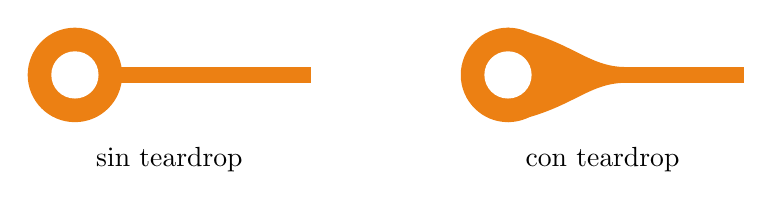
\begin{tikzpicture}[x=1cm,y=1cm]
  \begin{scope}
    \fill[orange!70!brown] (0,0) circle (0.6);
    \fill[white] (0,0) circle (0.3);
    \fill[orange!70!brown] (0.5,-0.1) rectangle (3,0.1);
    \node[below] at (1.2,-0.8) {sin teardrop};
  \end{scope}
  \begin{scope}[xshift=5.5cm]
    \fill[orange!70!brown] (0,0) circle (0.6);
    \fill[orange!70!brown] (0,0.6) .. controls (0.8,0.45) and (1.0,0.1) .. (1.5,0.1) -- (1.5,-0.1)
       .. controls (1.0,-0.1) and (0.8,-0.45) .. (0,-0.6) -- cycle;
    \fill[white] (0,0) circle (0.3);
    \fill[orange!70!brown] (1.45,-0.1) rectangle (3,0.1);
    \node[below] at (1.2,-0.8) {con teardrop};
  \end{scope}
\end{tikzpicture}
\caption{Unión de una pista con una vía, sin y con teardrop (dibujo ilustrativo).}
\label{fig:c06-teardrop}
\end{figure}

\textbf{Para qué sirve:}
\begin{itemize}
  \item \textbf{Tolerancia del taladro.} Si la broca cae corrida hacia el lado de la pista, puede cortar justo el
        punto donde la pista toca el anillo. Con la gota, sigue habiendo cobre a los lados.
  \item \textbf{Esfuerzo mecánico y térmico.} La esquina entre pista y pad concentra esfuerzos cuando la placa se
        calienta al soldar o se dobla un poco. Una transición suave los reparte.
\end{itemize}

\textbf{Cómo se hizo:} el script \archivo{tools/ruteo/teardrops.py} activa los teardrops en todos los pads que
tienen red y en todas las vías, con los parámetros por defecto de KiCad 10 (largo de la gota \num{0.5} veces el
tamaño del pad, como máximo \SI{1}{\milli\meter}; alto igual al tamaño del pad, como máximo \SI{2}{\milli\meter};
leídos en \archivo{pcb.kicad_pro}). KiCad
guarda cada teardrop como una pequeña zona de cobre. No hizo falta abrir la interfaz gráfica: el comando
\texttt{kicad-cli pcb drc --refill-zones --save-board} genera las zonas al rellenar. En la placa final hay
\textbf{440 zonas teardrop}, y el DRC sigue en 0. Los teardrops se agregan \emph{al final}, después de todo el ruteo,
porque cualquier cambio de pista obligaría a regenerarlos.

\begin{ojo}[los teardrops y la regla de entrada al pad]
La regla del dueño pide que las pistas entren al pad por el centro y en línea recta. Los teardrops no cambian eso:
se dibujan alrededor de la pista que ya entra recta. Por eso el chequeo propio (\archivo{revisar_pistas.py}) se corre
antes y después de agregarlos, y da 0 hallazgos en los dos casos.
\end{ojo}

% =====================================================================================================
\section*{Resumen}
\begin{itemize}
  \item Las reglas de fabricación salen de las tolerancias de cada paso: grabado, taladro, máscara, serigrafía y
        fresado.
  \item Los mínimos de JLC van solo como piso en KiCad. El diseño usa valores mayores: pistas de
        \SI{0.2}{\milli\meter} (el doble del mínimo), vías de 0.6/0.3 con anillo de \SI{0.15}{\milli\meter} (tres veces
        el mínimo), cobre a \SI{0.5}{\milli\meter} del borde.
  \item En 4 capas JLC tapona las vías, y una vía taponada debe estar a \SI{0.35}{\milli\meter} de los pads: se
        movieron 43 vías y se creó la regla \net{via_tapada_lejos_de_pad}. Los Gerber muestran 0 aperturas de
        máscara sobre las 329 vías.
  \item La placa va en PCBA \emph{Economic}. Como algunas piezas quedan a menos de \SI{2.5}{\milli\meter} del borde,
        JLC agrega los rieles; la placa trae 3 fiduciales.
  \item 4 capas, \SI{1.6}{\milli\meter}, verde y HASL sin plomo aparece en la tabla de \emph{Economic}. Falta
        confirmar en el formulario cuántas placas deja ensamblar.
  \item En KiCad hay tres niveles: piso de la placa, clases de red (valores de diseño) y 14 reglas propias en
        \archivo{pcb.kicad_dru}, cada una probada con una regla de control. Ningún chequeo quedó en ``ignorar''.
  \item Los teardrops (440) se generaron al final con \texttt{kicad-cli}, sin abrir la interfaz gráfica.
\end{itemize}
